
\clearpage
%\setcounter{page}{1}

\maketitlesupplementary

%\title{Reevaluation of Foundation Models in \\"Geography-Aware Self-Supervised Learning”}{Supplementary Material}
\section*{UMAP Feature Visualization} 

\vspace{10pt}
\begin{minipage}{\textwidth}
    The following figures visualize the UMAP features of the BigEarthNet-S2 test data's feature vectors extracted by the four re-evaluated foundation models.  The feature vectors that correspond to the specified class are shown in blue. This visualization is provided for each of the 19 labels. \\
\end{minipage}

\begin{figure}[htbp]
  \centering
   \begin{minipage}{\textwidth}
   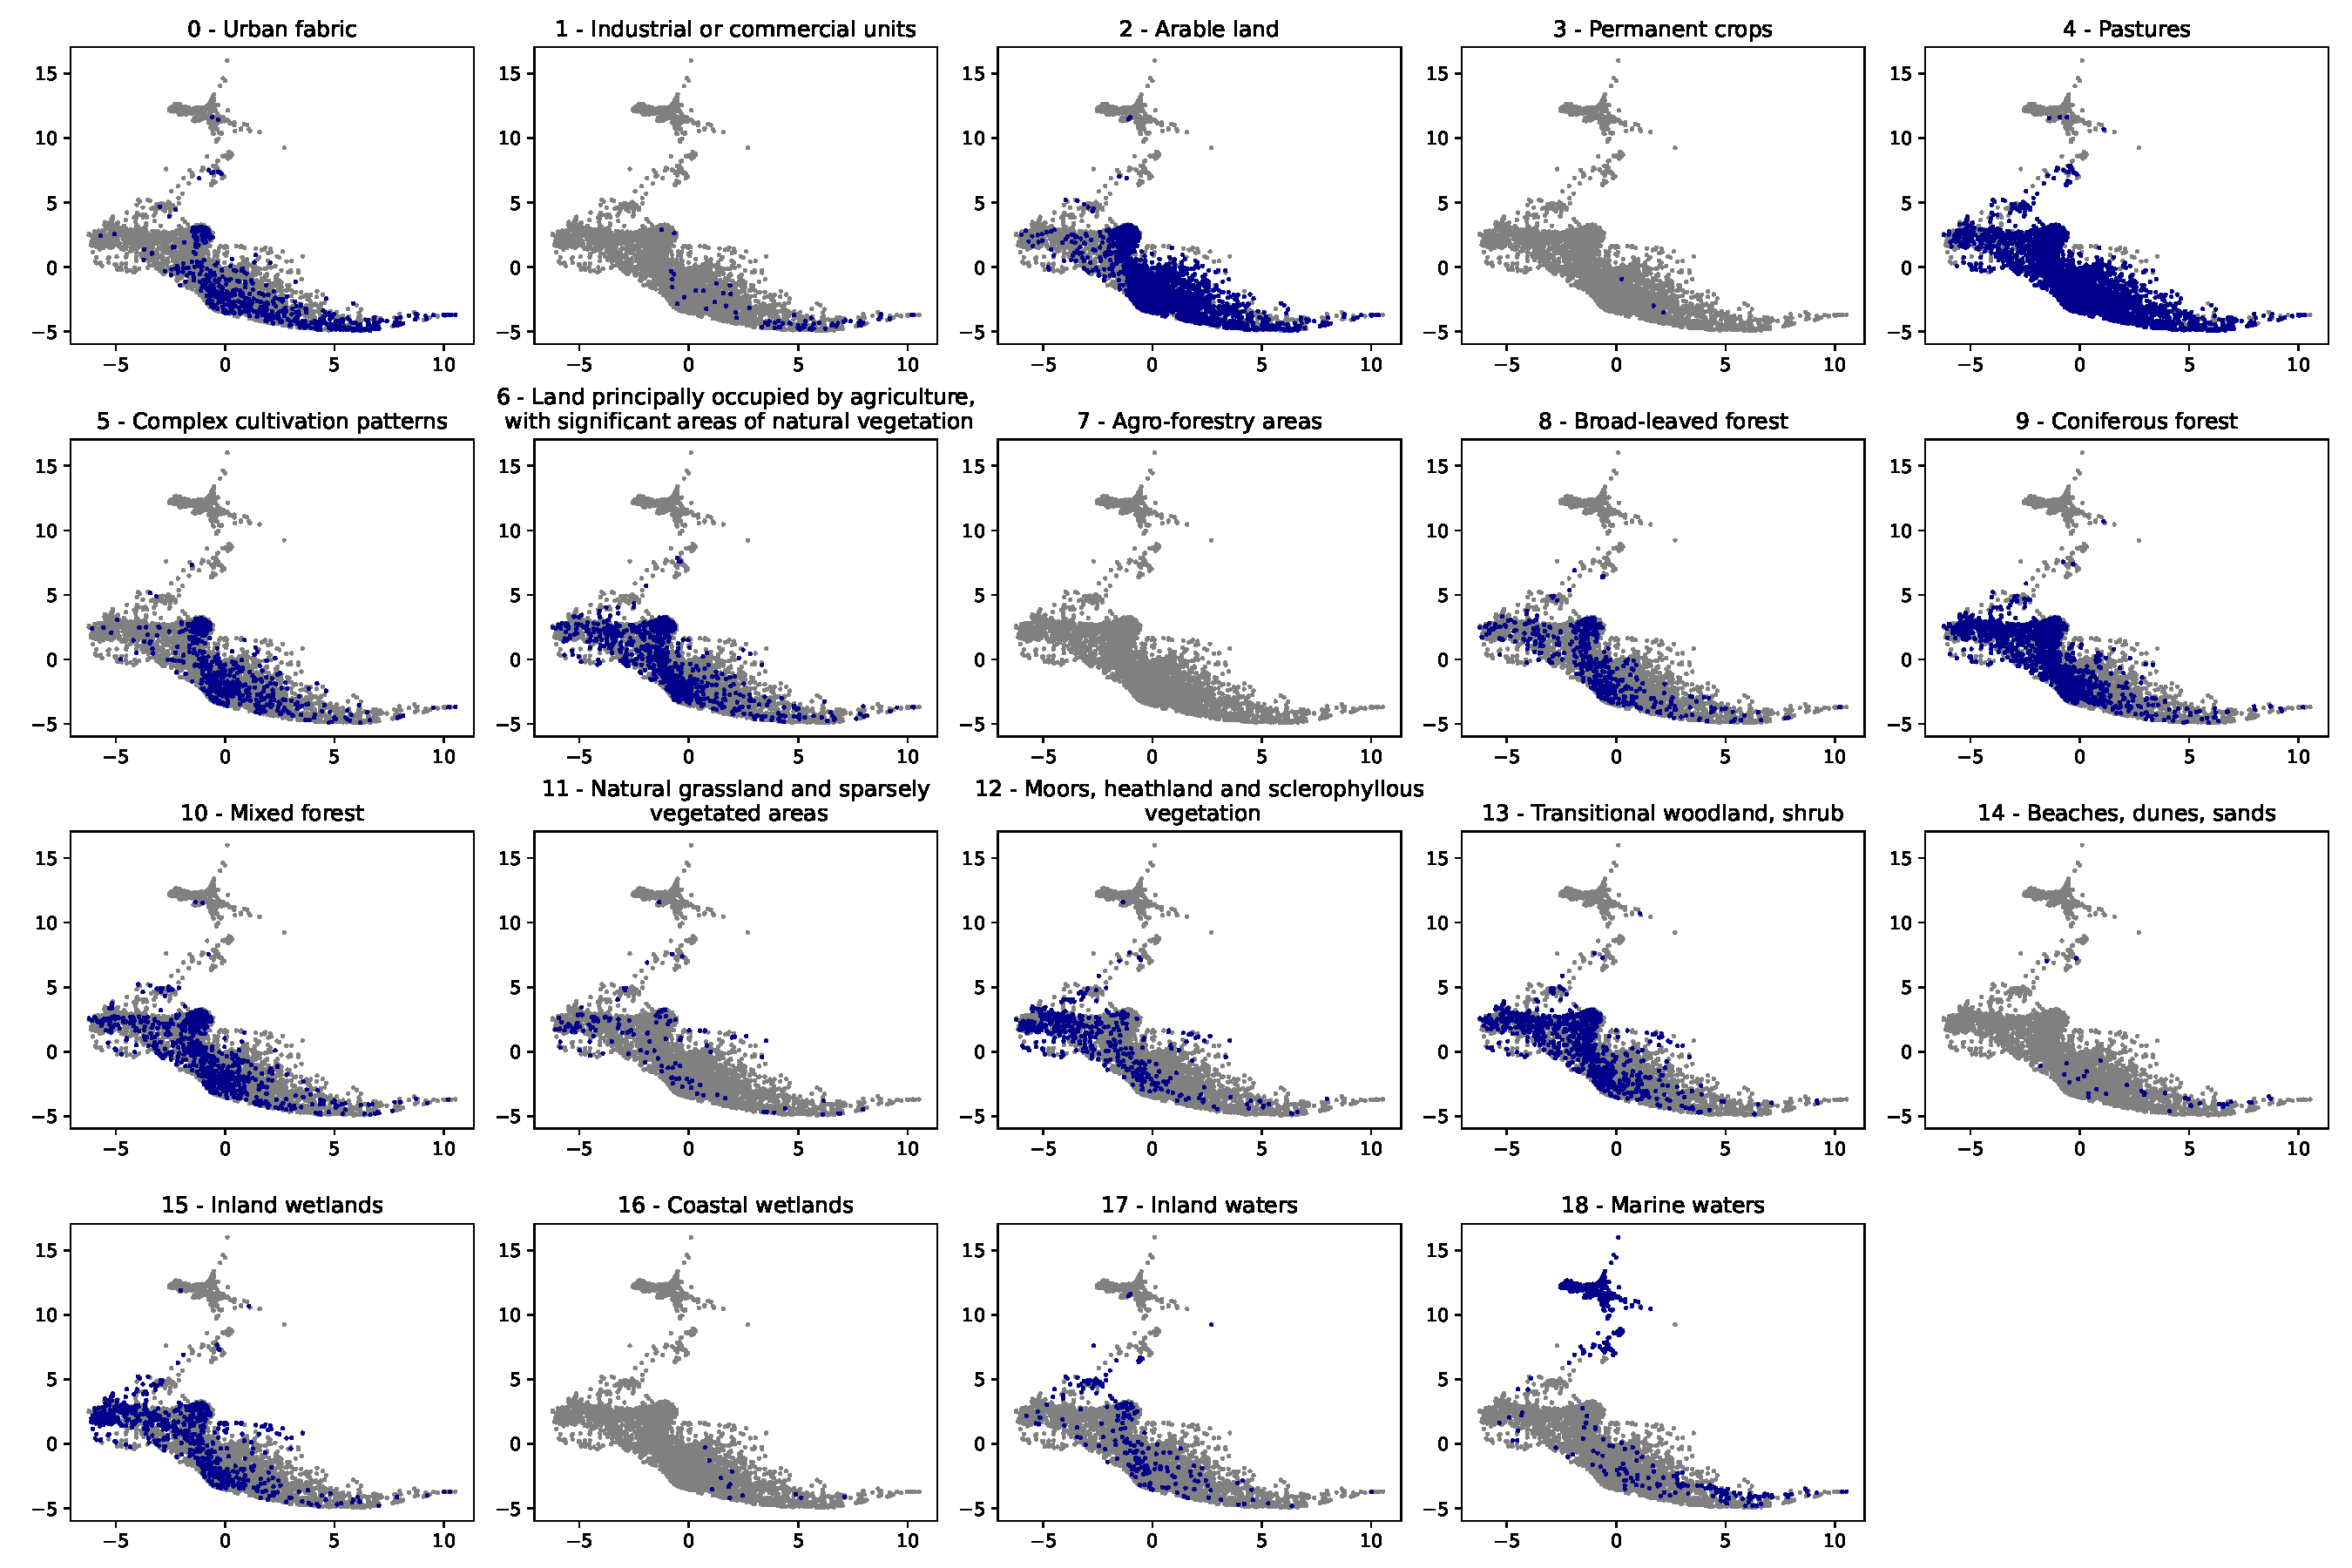
\includegraphics[width=\linewidth]{figures/all_labels_moco.pdf}
   %\captionsetup{justification=raggedleft, width=1.4\textwidth} #
   %\captionsetup{width=\linewidth} 
   %\vspace{2pt}
   \caption{MoCo-v2 foundation model.}
   \end{minipage}
\end{figure}

\begin{figure*}[htbp]
  \centering
   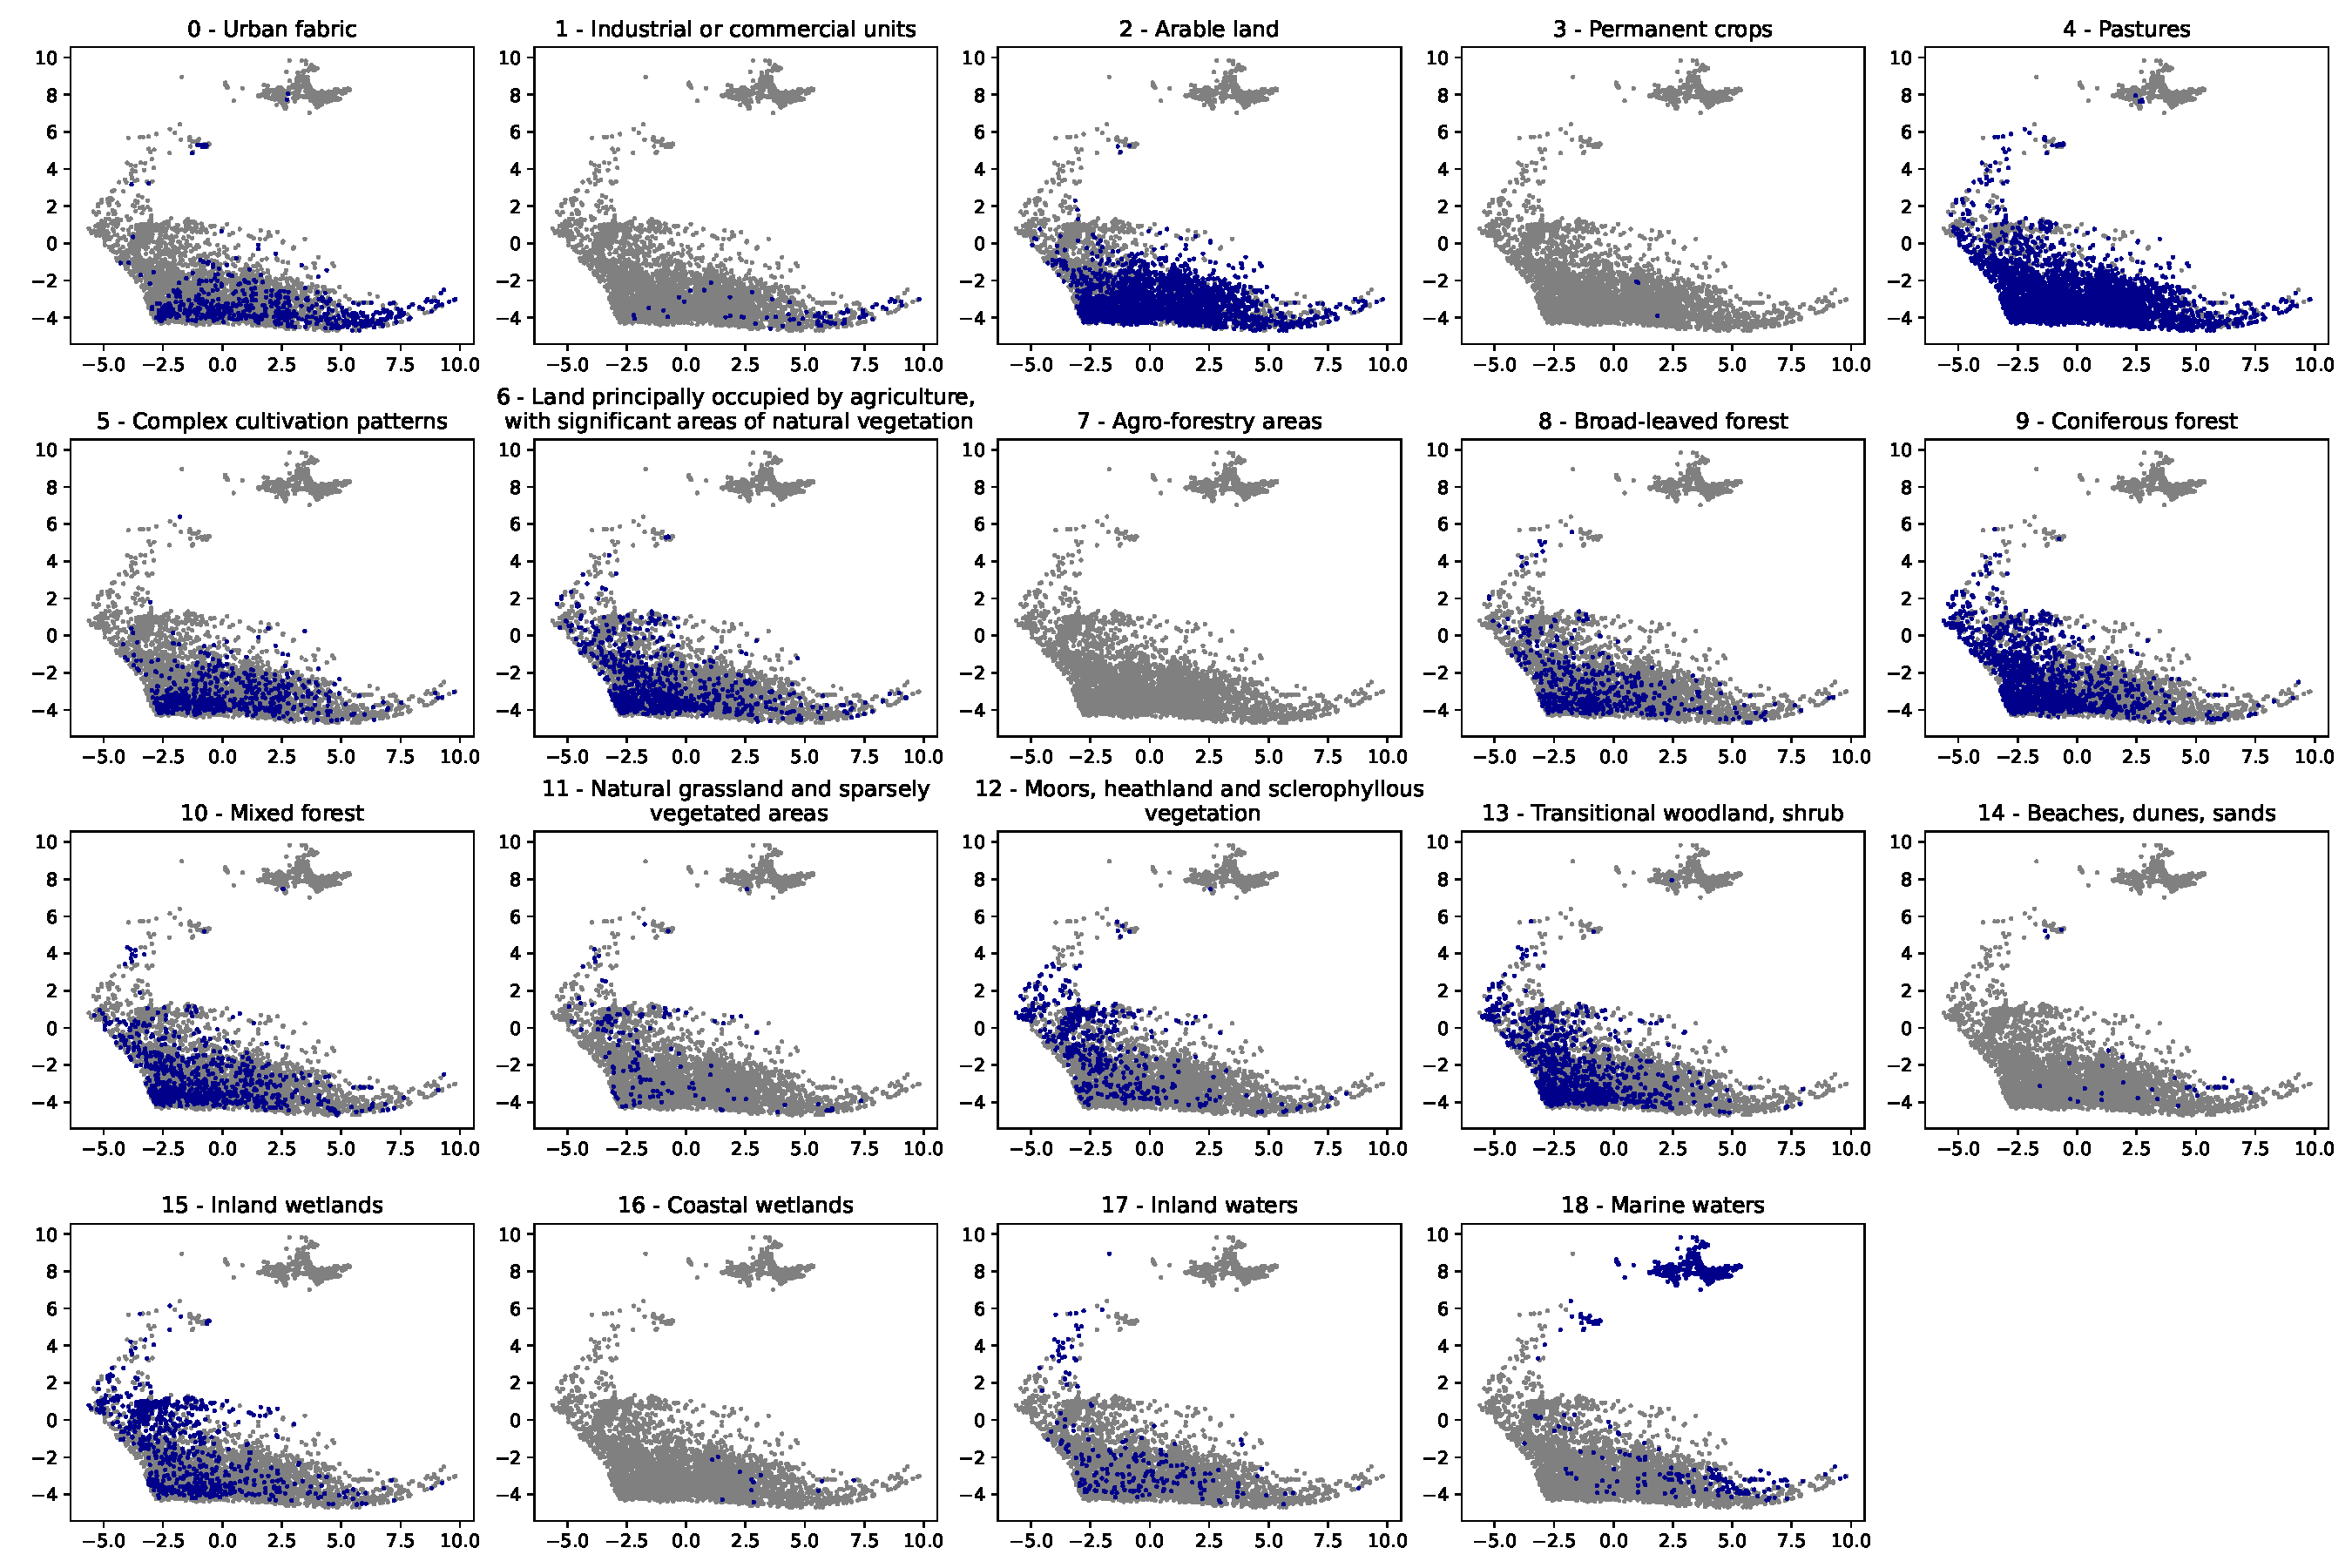
\includegraphics[width=\linewidth]{figures/all_labels_geo.pdf}
   \caption{MoCo-v2 additionally pre-trained on the geo-location classification task.}
\end{figure*}

\begin{figure*}[htbp]
  \centering
   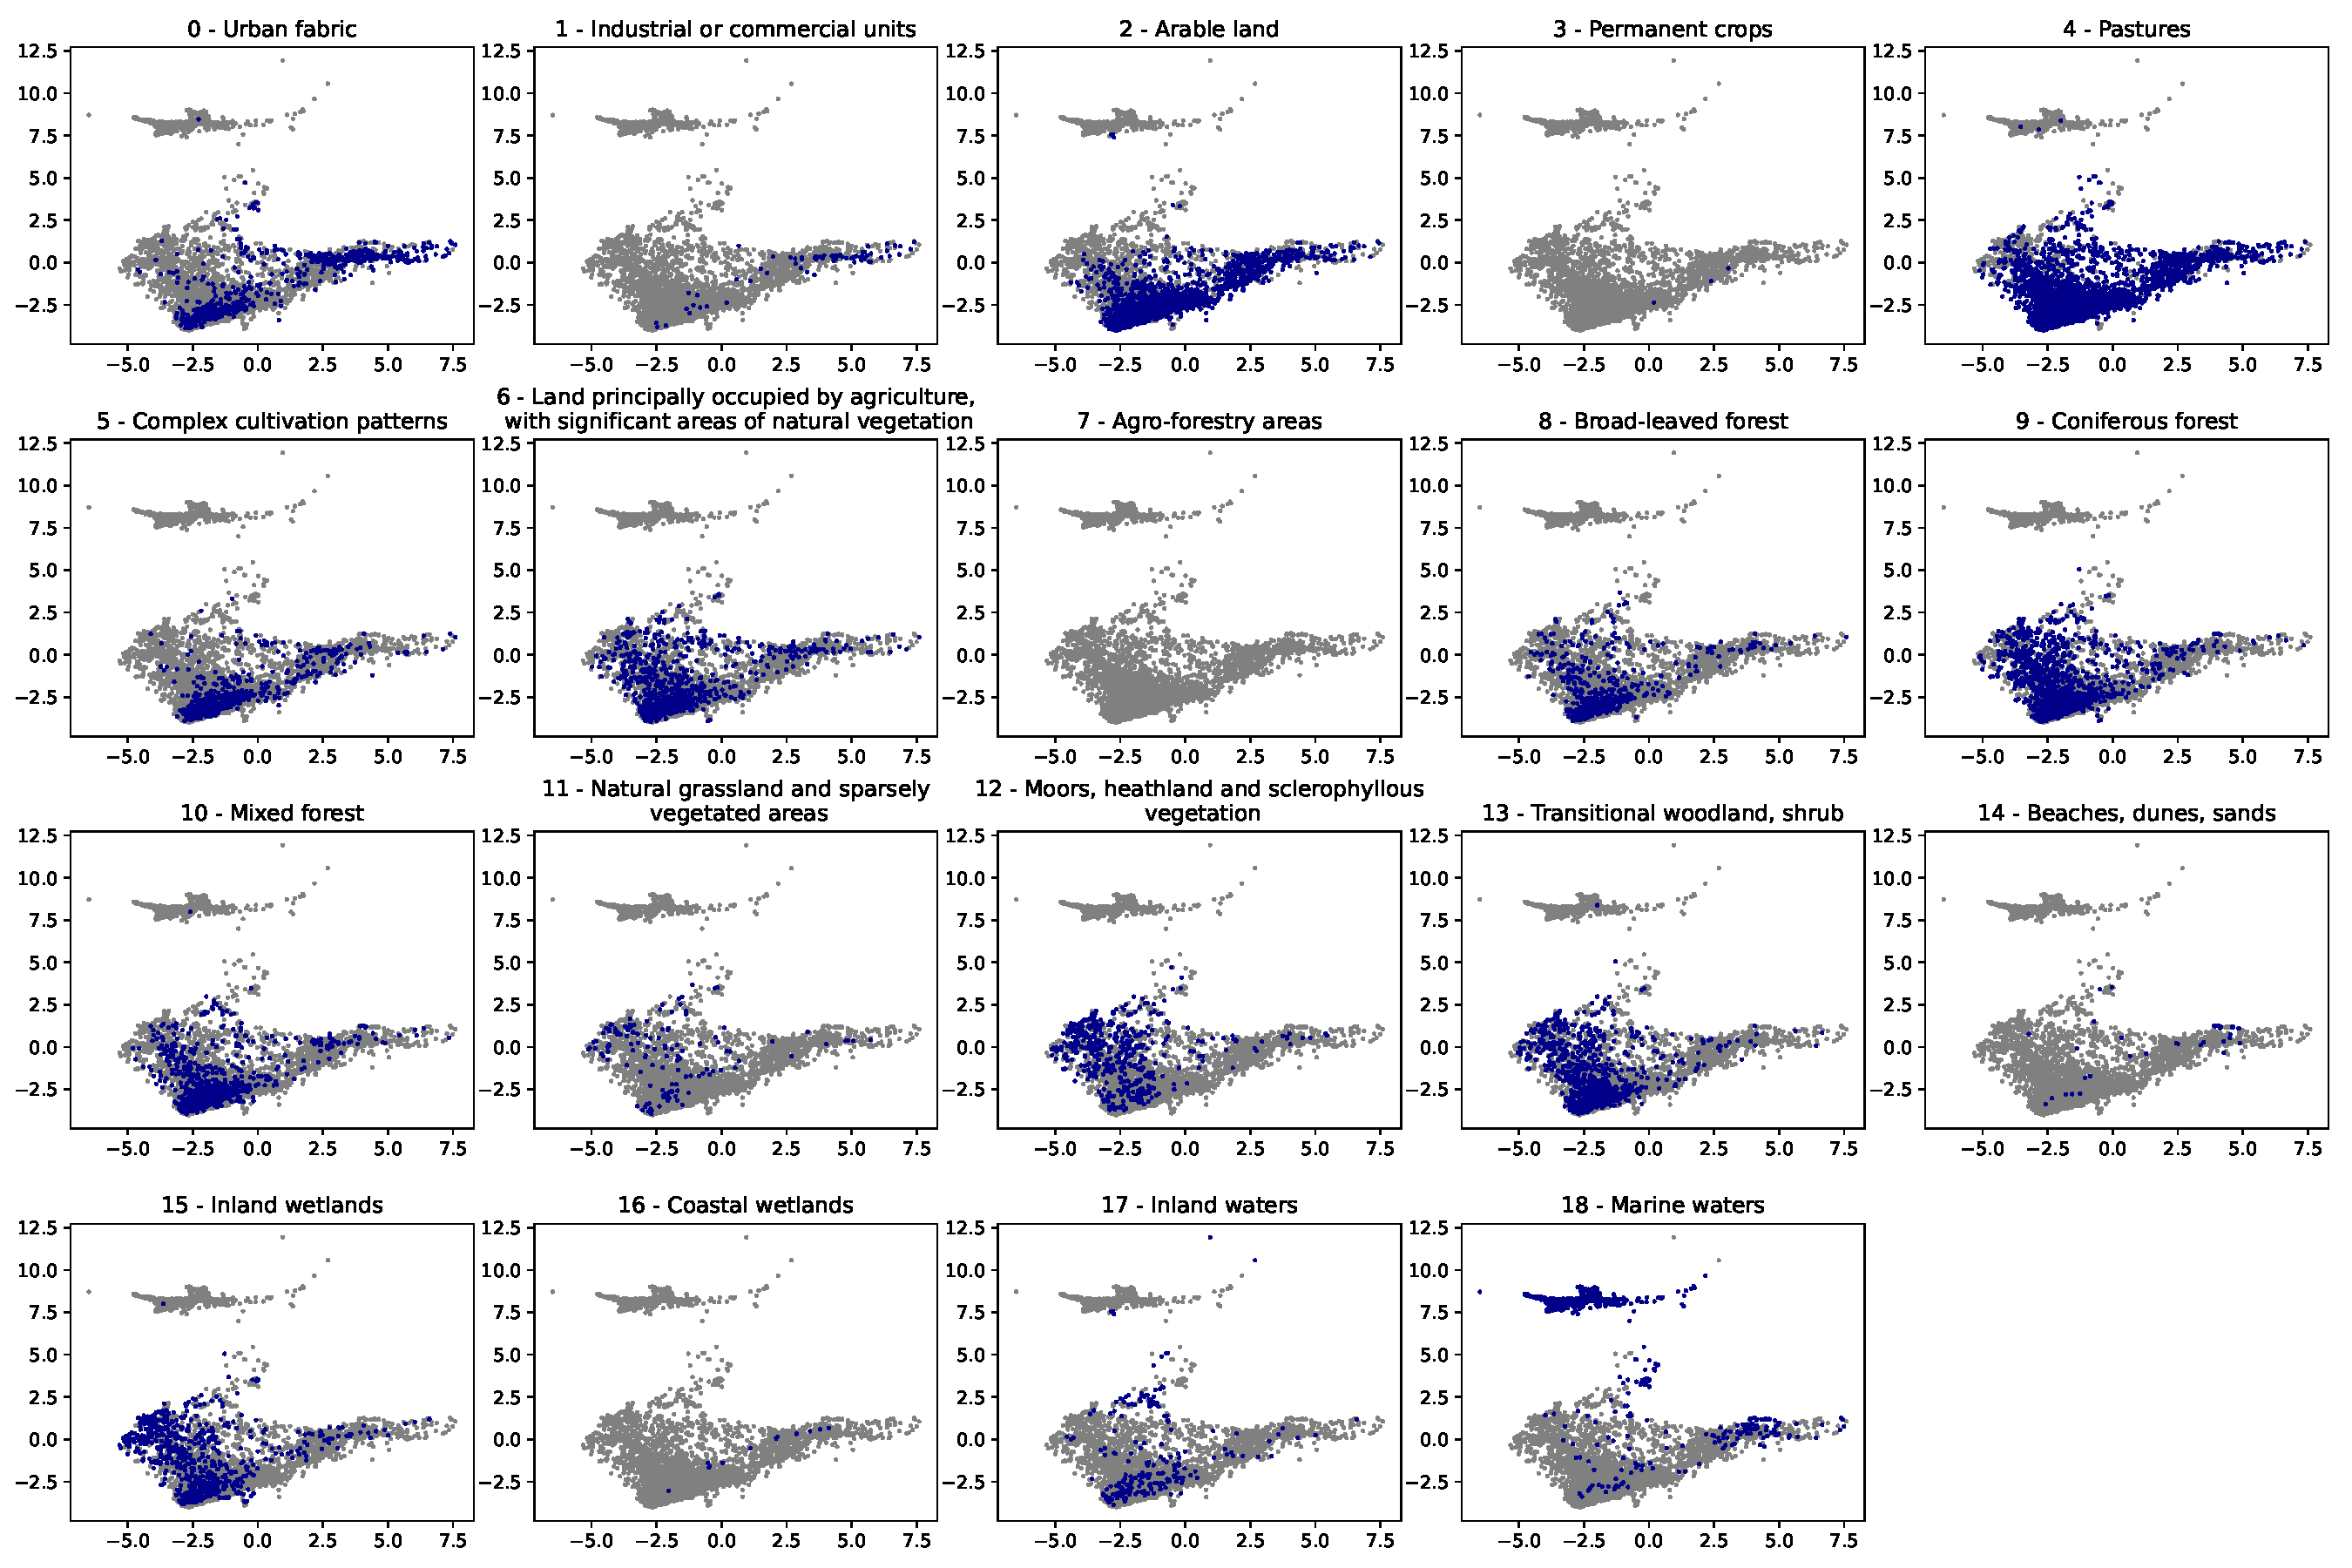
\includegraphics[width=\linewidth]{figures/all_labels_tp.pdf}
   \caption{MoCo-v2 trained with temporal positives.}
\end{figure*}

\begin{figure*}[htbp]
  \centering
   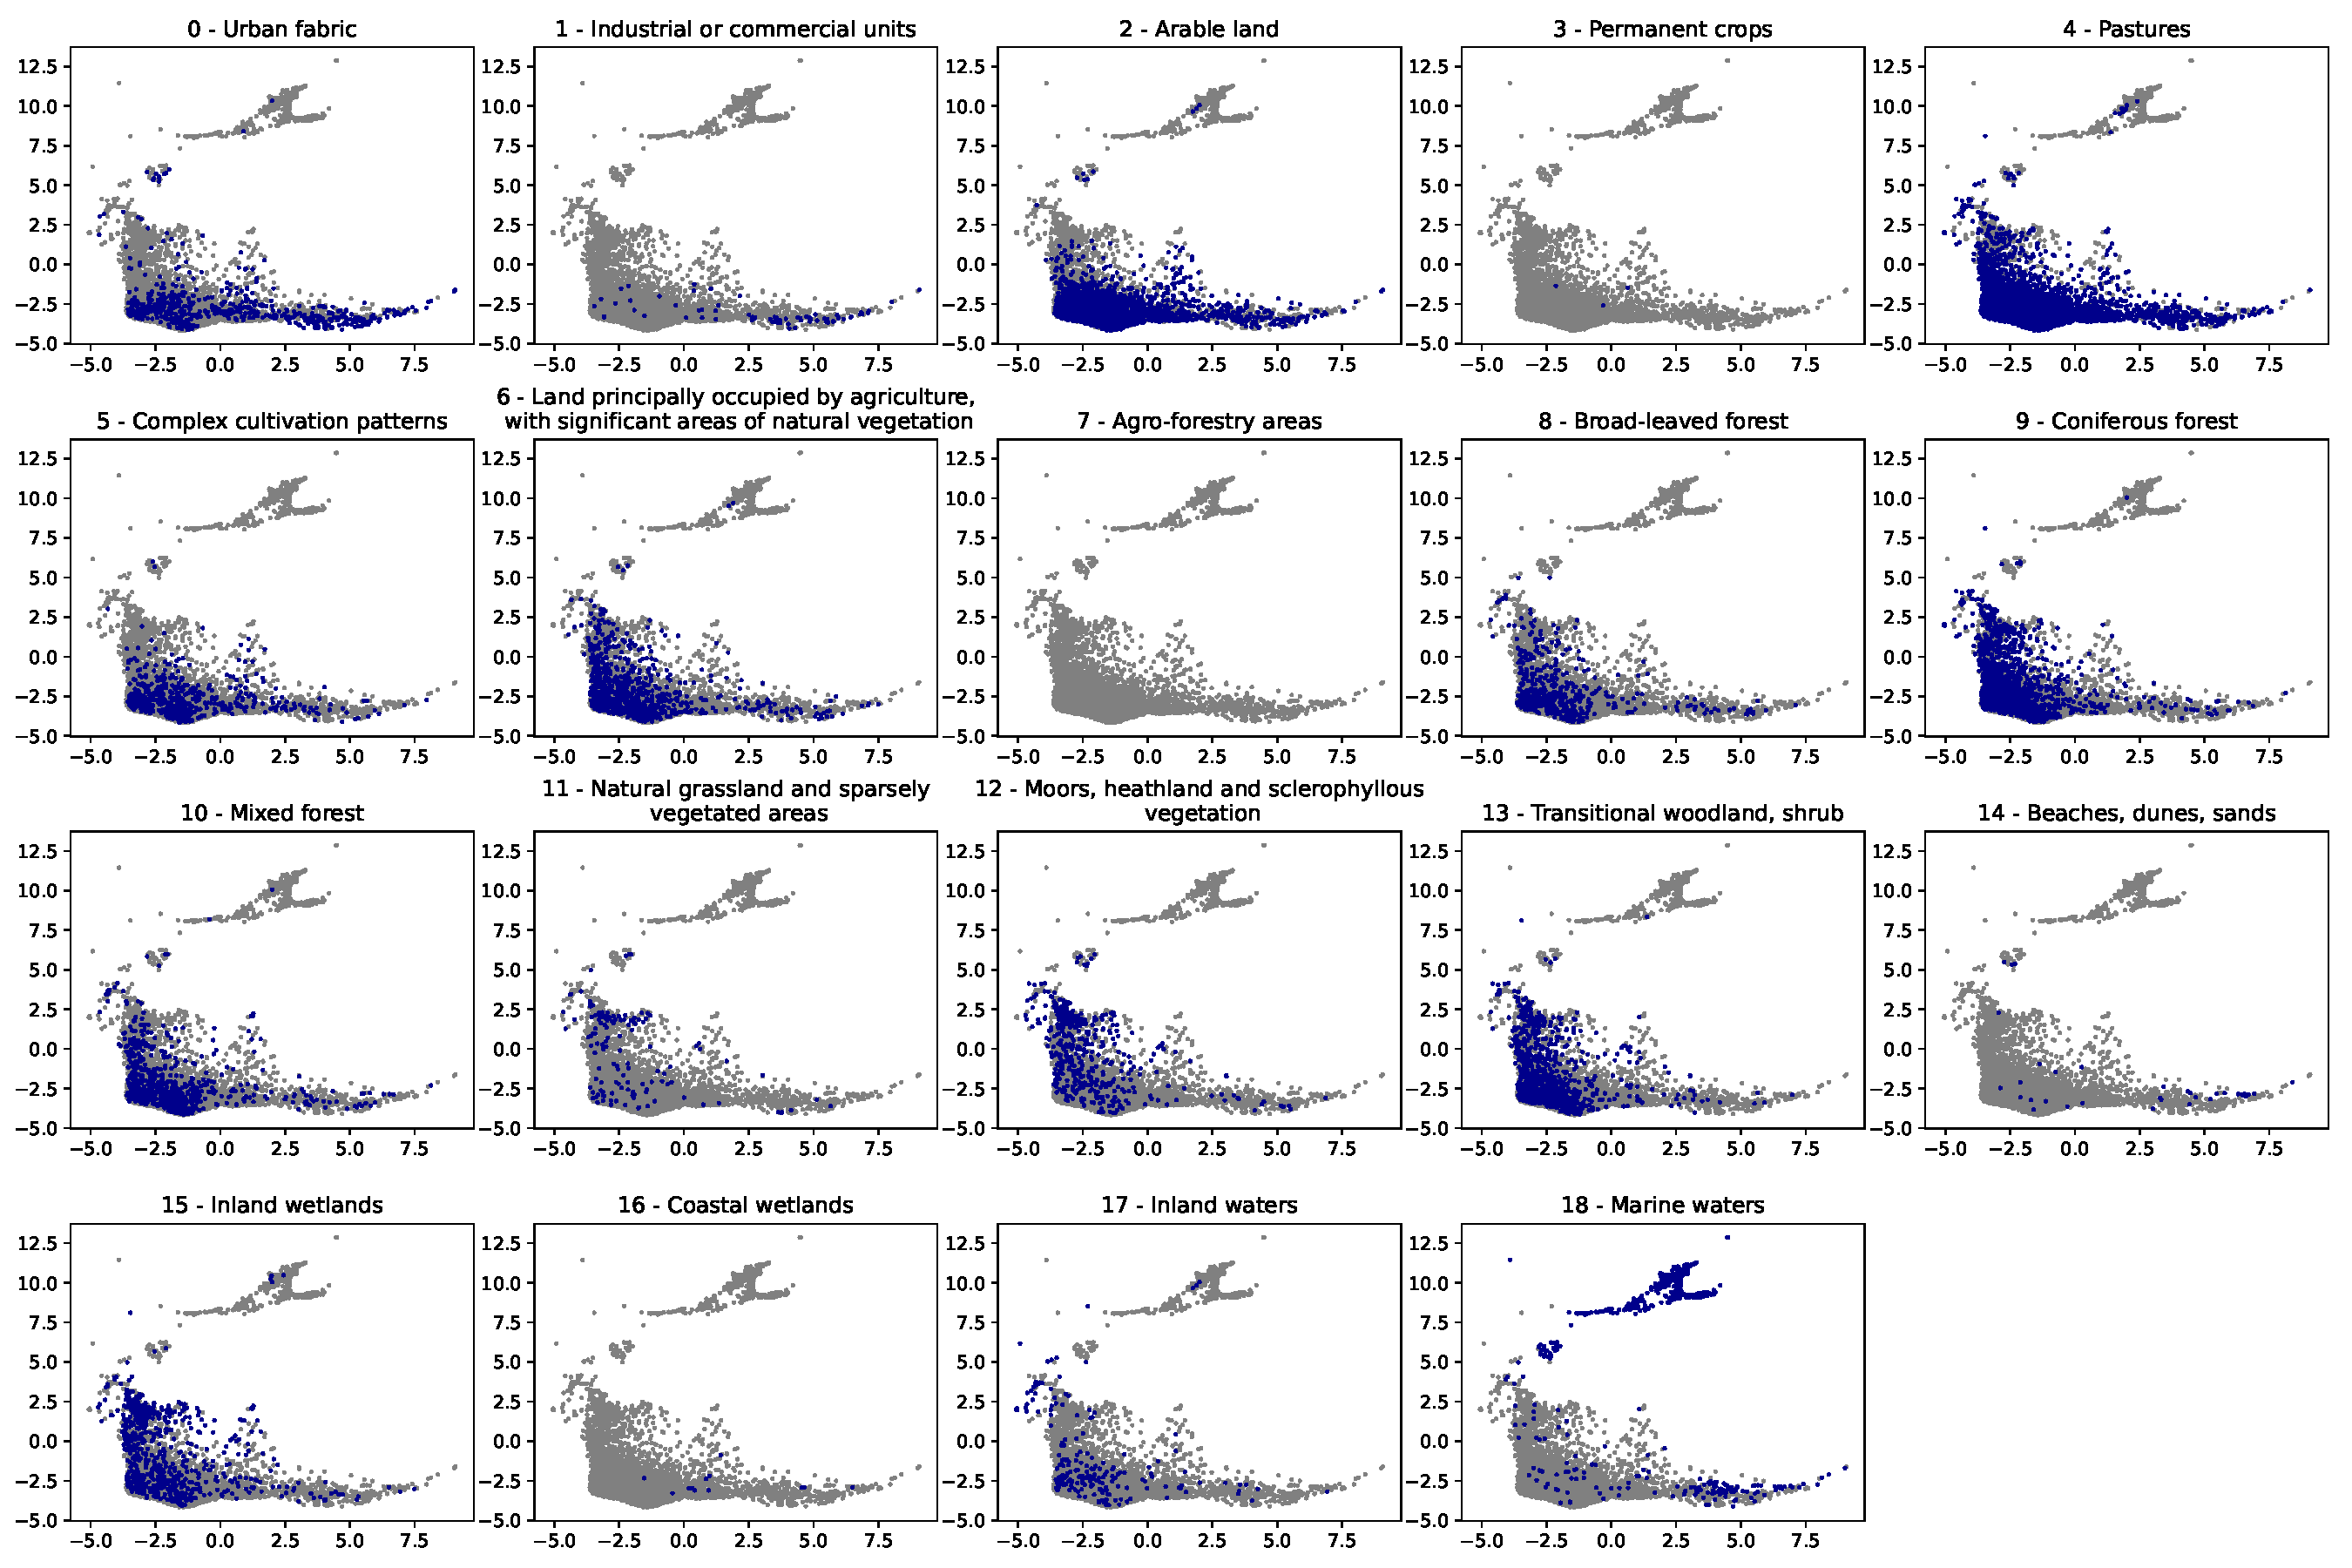
\includegraphics[width=\linewidth]{figures/all_labels_geo+tp.pdf}
   \caption{MoCo-v2 trained with temporal positives and on the geo-location classification task.}
\end{figure*}
